\documentclass[../main.tex]{subfiles}

\chapter{Wichtige Hinweise}
\label{c:intro}

Hier sind einige wichtige Hinweise zur Verwendung dieser Vorlage zusammengefasst, die erfahrungsgemäß oft falsch gemacht werden.
Fehler bitte an jochen.schmidt@fh-rosenheim.de melden.


%%%%%%%%%%%%%%%%%%%%%%%%%%%%%%%%%%%%%%%%%%%%%%%%%%%%%%%%%%%%%%
\section{Abbildungen und Tabellen}
\label{s:intro:abc}

Da dies leider immer wieder falsch gemacht wird (mit erheblichen Auswirkungen auf das Layout), hier einige Hinweise zur Positionierung von Bildern und Tabellen.
Im professionellen Textsatz werden diese als Gleitobjekte behandelt.
Wie der Name impliziert, bedeutet dies, dass Abbildungen (und Tabellen) relativ unabhängig vom Text platziert werden.
Insbesondere sollten Sie Latex \emph{niemals} dazu zwingen, Bilder genau an der von Ihnen vorgegebenen Stelle zu positionieren (z.\,B.\ mit Positionsangaben wie [h] oder schlimmer [h!]).
Es gibt dann für Latex keine Freiheit mehr, den Text richtig zu setzen, was unschöne Lücken zur Folgen hat.
Zudem wird durch ein Platzieren mitten im Text der Lesefluss unterbrochen.

%\begin{shaded*}
Gleitobjekte sollten daher immer mit [t] oder [tb] positioniert werden, oder bei großen Bildern auf Einzelseiten bzw.\ wenn mehrere Objekte auf einer textfreien Seite gesammelt werden sollen mit [p], alternativ mit [tbp].
%\end{shaded*}

Falls dadurch Bilder immer weiter vom eigentlichen Text wegrutschen, dann ist das ein Hinweise darauf, dass Sie im Verhältnis zu den Bildern zu wenig erläuternden Text geschrieben haben \dots

Jede Abbildung erhält eine Abbildungsnummer und eine Bildunterschrift.
Diese sollte kurz beschreiben, was in der Abbildung zu sehen ist und zu verstehen sein, ohne dass man den gesamten Text gelesen hat.
Jede Abbildung wird im Text beschrieben und referenziert, und zwar über die Abbildungsnummer, also z.\,B.\  "`Wie in Abb.\ 3.1 zu sehen ist \dots"'.
Nicht zulässig ist z.\,B.\ "`Wie in der folgenden Abbildung zu sehen ist \dots"' -- es gibt keine "`folgende"' Abbildung!
Ferner sollte darauf geachtet werden, dass alle Abbildungen/Tabellen gut lesbar sind.


\begin{figure}[t]
\centering

\begin{subfigure}{0.35\linewidth}
\centering
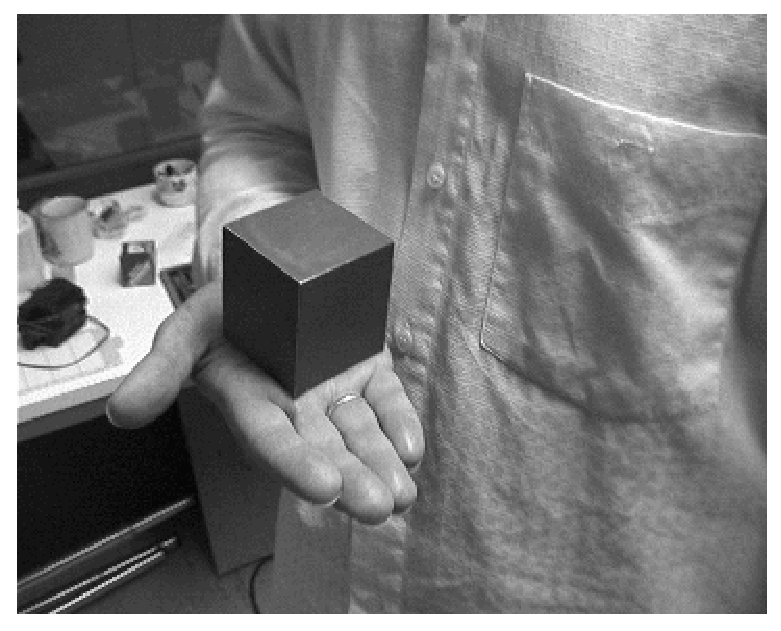
\includegraphics[width=\linewidth]{\figdir/handorig}
\caption{Originalbild}
\label{FIG:arexorig}
\end{subfigure}
\hspace{1cm}
\begin{subfigure}{0.35\linewidth}
\centering
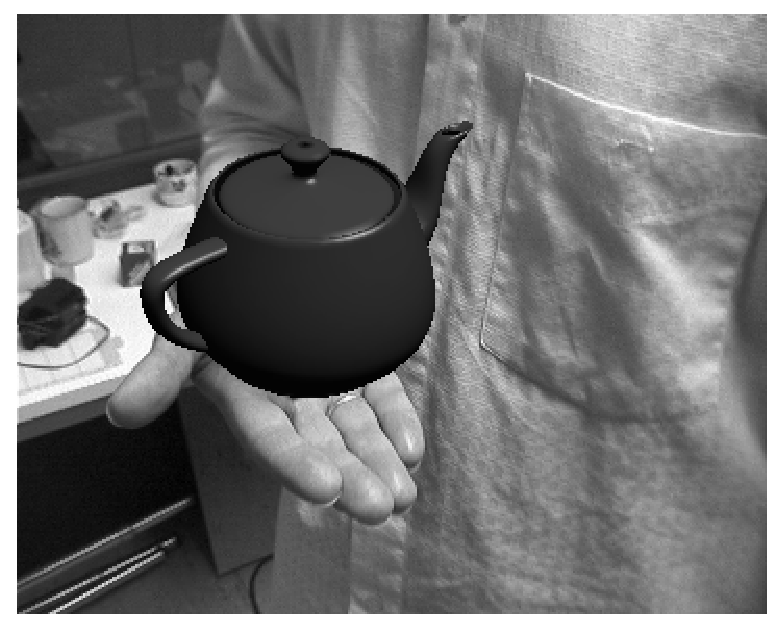
\includegraphics[width=\linewidth]{\figdir/handaug}
\caption{erweitertes Bild}
\label{FIG:arexaugm}
\end{subfigure}
%
\caption[AR Beispiel]
{Beispiel für Bilder, mit Beschreibung. Für nicht selbst erstellte Bilder, die nicht Public Domain sind, ist eine Quellenangabe erforderlich. Bilder aus \cite{Schmidt01:PAO}}
\label{FIG:arex}
\end{figure}

Ein Beispiel wird in Abb.\ \ref{FIG:arex} gezeigt, mit zwei Teilen  bestehend aus Abb.\ \ref{FIG:arexorig} und \ref{FIG:arexaugm}.
Und ein Beispiel für das Einbinden einer Tabelle, zu sehen in Tabelle \ref{t:CodebookOverview}.

\begin{table}[t]
\centering\small
 \caption[Testtabelle]{Datenselektion für verschiedene Testdatensätze}
  \label{t:CodebookOverview}
%
% generated by TexTableGenerator.pl ((c) Florian Vogt)
% from file: /home/Jochen/data/dissdata/results/CodebookOverview.log
%
\begin{tabular}{l|ccc|cc}
\hline
\hline
                  \textbf{Sequence} &          ARTS &           wman &         stcams &         ARTVZ &        ARTSUZ \\ 
                 \textbf{\# Frames} &             190 &              40 &             400 &             270 &             190 \\ 
     \textbf{\# relative movements} &           17955 &             780 &           79800 &           36315 &           17955 \\ 
\textbf{\# movements after pre-sel.} &           14336 &             623 &           37915 &           21788 &           14343 \\ 
       \textbf{min.\ angle in seq.} &   0.233$^\circ$ &    5.95$^\circ$ &   0.154$^\circ$ & 0.00000171$^\circ$ &  0.0388$^\circ$ \\ 
       \textbf{max.\ angle in seq.} &    81.7$^\circ$ &     180$^\circ$ &    47.3$^\circ$ &    80.3$^\circ$ &    80.9$^\circ$ \\ 
\textbf{min.\ angle after pre-sel.} &    12.9$^\circ$ &    21.1$^\circ$ &    17.3$^\circ$ &    16.3$^\circ$ &    12.9$^\circ$ \\ 
\textbf{max.\ angle after pre-sel.} &    81.7$^\circ$ &     161$^\circ$ &    47.3$^\circ$ &    80.3$^\circ$ &    80.9$^\circ$ \\ \hline\hline
\textbf{max.\ angle after pre-sel.} &    81.7$^\circ$ &     161$^\circ$ &    47.3$^\circ$ &    80.3$^\circ$ &    80.9$^\circ$ \\ \hline\hline
\end{tabular}

\end{table}

Bei Bildern verwendet man üblicherweise eine Bildunterschrift (also caption  unter dem Bild), bei Tabellen steht die Beschriftung üblicherweise über der Tabelle, da diese von oben nach unten gelesen werden.

Sind die Bilder/Tabellen schmal, kann die Beschriftung stattdessen auch neben dem Bild stehen.
Dies ist in Abb.\ \ref{fig:beschreibung-neben-bild} zu sehen (für ein Bild), verwendet wurde der Befehl fcapside.
Entsprechend funktioniert dies für Tabellen mit tcapside.
Die Einstellungen wurden so gewählt, dass die Beschriftung immer an der Innenseite ist (für doppelseitigen Druck).
Für eine korrekte Darstellung sind evtl.\ mehrere Latex-Läufe nötig.


\section{Seitenumbrüche}
Überlassen Sie Seitenumbrüche Latex, verwenden Sie kein newpage oder pagebreak.
Diese Befehle sind nur in sehr wenigen Ausnahmefällen erforderlich.
Wenn Sie diese verwenden müssen ist dies eher ein Hinweis darauf, dass etwas anderes mit Ihrem Layout nicht stimmt.

\section{Schriftart}
Als Schriftart für den Haupttext ist Palatino voreingestellt.
Dies hat in erster Linie zwei Gründe:
\begin{enumerate}
\item
Die Schrift ist etwas breiter als z.\,B.\ Times und daher gerade für den A4-Druck (zur besseren Lesbarkeit) noch am besten geeignet.
\item
Es gibt einen passenden Mathematikzeichensatz dazu, d.\,h.\ Ziffern und Buchstaben (wenn beide gerade bzw.\ kursiv gedruckt werden) sehen im Text und im Mathemodus gleich aus -- alles andere wäre unschön.
\end{enumerate}
Passende Mathematikzeichensätze gibt es auch für Times und Computer/Latin Modern, die stattdessen verwendet werden können.
Kommentieren Sie in diesem Fall das Paket mathpazo (durch ein \%) aus, und dafür lmodern (für Latin Modern) oder mathptmx (für Times) ein.

Weitere Hinweise zu den Themen Seitenlayout/Einfluss der Schriftart findet man z.\,B.\ in der Dokumentation zu KomaScript\footnote{\url{http://www.komascript.de}}.


\section{Druck}
Die Vorlage ist für doppelseitigen Druck eingerichtet, den Sie auch verwenden sollten.
Wenn (aus welchem Grund auch immer) ein einseitiger Druck erwünscht ist, schalten Sie die Vorlage bitte um: Ganz oben in thesis.tex muss dann aus twoside=true ein twoside=false werden.
Wird dies  nicht beachtet erscheinen die Seitenzahlen einmal innen und einmal außen, zudem entstehen komplett leere Seiten (die beim doppelseitigen Druck Rückseiten wären, die dazu dienen, dass ein neues Kapitel auf einer rechten Seite anfängt).
Wenn Sie die Arbeit nicht selbst drucken, denken Sie daran, den Dienstleister auf den doppelseitigen Druck hinzuweisen.



\section{Dokument Richtlinien}
Beachten Sie bitte auch die Hinweise im separaten Dokument "`Hinweise zur Erstellung von Abschlussarbeiten"'.

\section{Diverse Beispiele}

Verwenden Sie für Querverweise den Befehl label und  ref (Bilder und Tabellen), eqref (Formeln), pageref (Seitenzahlen) damit diese automatisch erzeugt werden.
Beachten Sie vor der Abgabe der Arbeit, dass evtl.\ mehrere Latexläufe erforderlich sind, bis alle Querverweise korrekt sind, da Latex diese während eines Laufs erzeugt und beim nächsten wieder einliest.
Durch Verschiebungen können je nach verwendeten Paketen auch drei oder vier Läufe erforderlich sein, bis alles passt.



Beispiel für eine Formel
\begin{equation}
\label{eq:cvp:test}
f(x) = \frac{1}{3} x + 5, \quad x \in \real.
\end{equation}

Und noch eine:
\begin{equation}
\label{eq:cvp:matvec}
\mathbf{M}  = \mathbf{Ax} \pi, \quad \mathbf{A} \in \real^{2 \times 2}, \mathbf{x} \in \real^2.
\end{equation}

Eine Referenz auf eine Formel: \eqref{eq:cvp:test}.

Und eine Literaturreferenz: \cite{Auer00:HTF}.
Verwenden Sie auf jeden Fall Bibtex (oder etwas äquivalentes), Referenzen sollten auf keinen Fall manuell eingefügt werden.

Gedankenstriche entstehen durch zwei Minuszeichen -- und sind länger als ein Bindestrich -.

Und wenn es ganz besonders schön aussehen, dann beachten Sie zusätzlich
\begin{itemize}
\item Der Leerraum nach eine Punkt am Satzende ist größer als der nach einer Abkürzung (wie evtl.). 
Um Latex zu sagen, dass der Punkt kein Satzende ist, wird dieser bei Abkürzungen durch einen Backslash markiert, also so: evtl.\textbackslash, ohne Leerzeichen zwischen Punkt und Backslash.

\item
Leerräume zwischen zwei Teilen einer Abkürzung (wie z.\,B.) sind kleiner als zwischen einzelnen Wörtern, außerdem sollten diese beiden Buchstaben nicht getrennt werden. Dies erreicht man durch: z.\textbackslash,B.\textbackslash, wieder ohne Leerzeichen.
\end{itemize}
Noch ein Hinweis zur Silbentrennung von Wörtern mit Bindestrichen: Diese werden nur direkt am Bindestrich getrennt (so soll es eigentlich sein), was insbesondere im Deutschen oft dazu führt, dass Wörter in den Rand hineinragen (man bekommt auch eine Overfull Box Warnung).
Möchte man, dass die Wörter selbst auch getrennt werden dürfen, so kann man
\begin{itemize}
\item
entweder bei Problemfällen manuelle Trennpunkte durch \textbackslash - in das Wort einfügen,
\item oder statt des Bindestrichs - die Zeichenfolge "'= verwenden, also wort"'=wort statt wort-wort.
\end{itemize}
In vielen Fällen sollte man sich zudem fragen, ob das Wort nicht eher zusammen geschrieben werden sollte (statt des Bindestrichs).


%%% Local Variables: 
%%% mode: latex
%%% TeX-master: "thesis.tex"
%%% End: 
